%---------------------------------------------------
% Nombre: capitulo1.tex  
% 
% Texto del capitulo 1
%---------------------------------------------------

\chapter{F�sica}

En esta quinta pr�ctica de la asignatura, a�adiremos comportamiento f�sico al modelo generado en la anterior pr�ctica, el cual podemos ver en la figura \ref{img_1}. Tambi�n realizaremos el tutorial de la asignatura \cite{guion} para familiarizarnos con los conceptos necesarios para la realizaci�n de la pr�ctica. 

\begin{figure}[H]
	\centering
		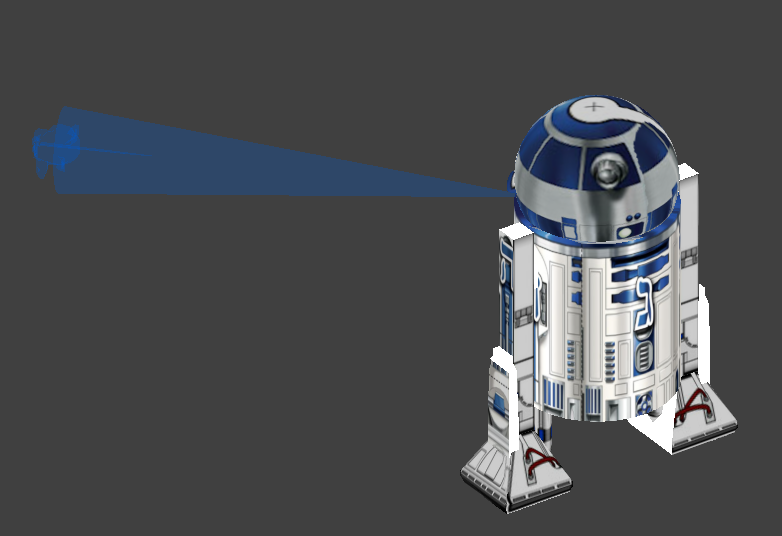
\includegraphics[scale=0.4]{./Capitulo1/Imagenes/holo.png}
		\caption{Modelo final de la pr�ctica anterior.}
	\label{img_1}
\end{figure} 


\section{Conclusiones}

El a�adir f�sica a nuestros modelos en blender, o a�adir�a a nuevos objetos que a�adamos para que las interacciones de nuestro modelo se asimilen a como serian en el mundo real, es uno de los conceptos m�s interesantes de Blender, aunque por otro lado, tambi�n ofrece en ciertos puntos una complejidad avanzada, debida en gran medida a la cantidad de par�metros disponibles en cuanto a \textb{f�sica} en nuestro modelo se refiere. 

\clearpage
%---------------------------------------------------